\documentclass[onecolumn,10pt]{article}
\usepackage[latin1]{inputenc}
\usepackage[a4paper,top=2cm, left=1.5cm, right=1.5cm, bottom=2cm, includefoot,includehead]{geometry}
\usepackage{graphicx}
\usepackage{amsfonts}
\usepackage{amsmath}
\usepackage{amssymb}
\usepackage[spanish]{babel}
\usepackage{apalike}
\usepackage{latexsym,amsmath,amssymb}
\usepackage{epstopdf}
\usepackage[section]{placeins}
\usepackage{graphicx}
\usepackage{booktabs}
\usepackage{makecell}
\usepackage{listings}
\spanishdecimal{.}

\title{Reporte de Actividades} 
\vspace{0.3cm} 
\author{Bartolo Garc\'ia Luis Enrique}
\date{03 de Noviembre del 2021}


\begin{document}
\twocolumn[
\begin{@twocolumnfalse}
\maketitle
\begin{center}
\rule{0.9\textwidth}{0.1mm}
\begin{abstract}
\begin{center}
Se entregar\'a el avance de los resultados obtenidos sobre las actividades asignadas relacionadas a la tesis.
\end{center}
\end{abstract}
\rule{0.9\textwidth}{0.1mm}
\end{center}
\end{@twocolumnfalse}
]

\section{Introducci\'on}
El sistema con el que se trabaj\'o es un levitador 

magn\'etico formado por un resistor conectado en serie con una bobina en el que debajo de ella se situa un objeto de masa $m[kg]$ hecho de material ferromagn\'etico, un controlador variar\'a el campo magn\'etico de la bobina lo que generar\'a una fuerza de atracci\'on sobre el objeto modificando su posici\'on vertical $r[m]$ respecto a esta.

\begin{figure}[h]
\centering
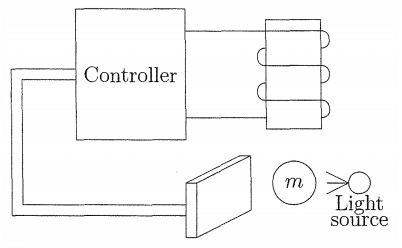
\includegraphics[scale=0.5]{levitador.png}
\caption{Levitador Magn\'etico}
\label{levitador}
\end{figure}

De acuerdo a la descripci\'on del funcionamiento del sistema se plantearon los siguientes objetivos:
\begin{itemize}
 \item Llevar al objeto antes mencionado a una posici\'on determinada sujeta a ciertas restricciones.
 \item Implementar controladores lineales como LQR, PD y PID.
 \item Aplicar controladores  no lineales basados en modos deslizantes.
 \item Obtener un sistema de orden reducido al que se le dise\~nar\'an sus propios controladores.
 \item Controlar al levitador con los controladores dise\~nados para el sistema de orden reducido.
 \item Aplicar perturbaciones al sistema para comparar el desempe\~no de los controladores implementados.
\end{itemize}
 

\section{Sistema de 3er Orden}
\subsection*{Representaci\'on del sistema}
El sistema est\'a determinado por 3 ecuaciones diferenciales que modelan la parte mec\'anica y la parte el\'ectrica:
\begin{itemize}
\item $m\ddot{y}+k\dot{y}+mg-F(y,i)=0$
\item $v=\dot{\phi}+Ri$
\item $\phi=L(y)i$
\end{itemize}



Donde $m$ es la masa del objeto, $y$ es la posici\'on vertical del objeto medida desde un punto de referencia ($y=0$ es justo debajo de la bobina), $k$ es el coeficiente de fricci\'on viscosa, $g$ es la aceleraci\'on debido a la gravedad, $i$ es la corriente el\'ectrica, $R$ es la resistencia el\'ectrica y $\phi$ es el flujo magn\'etico.
\\
\\
La funciones auxiliares $L(y)$ y $F(y,i)$  que modelan la inductancia y la fuerza  generada por la bobina respectivamente est\'an definidas por:
\begin{itemize}
\item $L(y)=L_1+\dfrac{L_0}{1+y/a}$
\item $F(y,i)=-\dfrac{L_0i^{2}}{2a(1+y/a)^{2}}$
\end{itemize}
Donde $L_0$,$L_1$ y $a$ son constantes positivas. 

\begin{table}[htbp]
\begin{center}
\begin{tabular}{|l|l|}
\hline
Par\'ametro & Valor \\
\hline \hline
$m$ & 0.1203 $[kg]$ \\ \hline
$k$ & 0.01 $[N.m/s]$\\ \hline
$R$ & 1.75$[\Omega]$\\ \hline
$L_0$ & 0.245 $[H]$ \\ \hline
$L_1$ & 0.1 $[H]$ \\ \hline
$g$ & 9.815 $[m/s^{2}]$ \\ \hline
$a$ & 0.0088 $[m]$ \\ \hline
\end{tabular}
\caption{Lista de Par\'ametros.}
\end{center}
\end{table}

Para lograr los objetivos planteados se elegi\'o una representaci\'on en espacio de estados del sistema donde 

$x_1=y$, $x_2=\dot{y}$, $x_3=i$ y $u=v$, dando como resultado un sistema de 3er orden que toma la siguiente forma:

$$
\dot{x_1}=x_2 
$$
$$
\dot{x_2}=-\dfrac{k}{m}x_2-g+\dfrac{aL_0x_3^{2}}{2m(a+x_1)^{2}}
$$
$$
\dot{x_3}=\dfrac{1}{L(x_1)}(-Rx_3+\dfrac{aL_0x_2x_3}{(a+x_1)^{2}}+u)
$$

Para llevar al objeto a una posici\'on de inter\'es y mantenerlo ah\'i los estados del sistema deben de tomar un conjunto de valores espec\'ificos $X_d$ debido a una entrada de valor $U_d$ que har\'an que $\dot{x}=0$, a este conjunto de valores se le conoce como punto de operaci\'on, para este sistema en concreto ser\'a:
$$
X_{D}=\begin{bmatrix}
X_{1_{D}} \\ 0 \\ \sqrt{\dfrac{2mg}{aL_0}(a+X_{1_{D}})^{2}} 
\end{bmatrix}
$$
$$
U_{d}=\begin{matrix}
R\sqrt{\dfrac{2mg}{aL_0}(a+X_{1_{D}})^{2}}
\end{matrix}
$$
$X_{1_{D}}$ es la distancia a la cual queremos situar el objeto y se eligi\'o $0.01[m]$, valor que se mantuv\'o constante para todas las actividades restantes, obteniendo lo siguiente:
$$
X_{D}=\begin{bmatrix}
0.01 \\ 0 \\ 0.6222 
\end{bmatrix}
$$
$$
U_{d}=\begin{matrix}
1.0888
\end{matrix}
$$

Teniendo en cuenta los objetivos planteados, m\'as adelante se agregar\'on perturbaciones constantes y variables al sistema, para ello se modificaron un poco las ecuaciones de estado anteriores:

$$
\dot{x_1}=x_2 
$$
$$
\dot{x_2}=-\dfrac{k}{m}x_2-g+\dfrac{aL_0x_3^{2}}{2m(a+x_1)^{2}}+f(t)
$$
$$
\dot{x_3}=\dfrac{1}{L(x_1)}(-Rx_3+\dfrac{aL_0x_2x_3}{(a+x_1)^{2}}+u)
$$

Donde $f(t)$ es una perturbaci\'on acotada que entra al sistema, de manera concreta se aplic\'o en la ecuaci\'on para $\dot{x_2}$ ya que en ella se expresan las aceleraciones que actuan sobre el objeto que es movido por la bobina, por lo que el termino $f(t)$ lo tender\'a a sacar de balance alterando la posici\'on a la que se le quiere llevar, con esto se quiso probar la robustez de los controladores empleados. 

\subsection*{An\'alisis del sistema}
Dejando de lado un momento el sistema perturbado y trabajando con el sistema original, el an\'alisis de estabilidad del punto de operaci\'on se realiz\'o mediante el M\'etodo Indirecto de Lyapunov (MIL), por lo que se requiri\'o linealizar al sistema para obtener una representaci\'on $\dot{x}=Ax+Bu$, $y=Cx+Du$, las matrices $A$, $B$, $C$ y $D$ se calculan obteniendo el jacobiano del sistema y valuandolo en $X_{d}$ y $U_{d}$.


Para facilitar el proceso se us\'o un modelo de Simulink junto con el comando linmode de MATLAB, con lo que se obtuvo el valor num\'erico de las matrices requeridas:

$$A=\begin{bmatrix}
0 & 1 & 0\\
-1044.1495 & -0.0831 & 31.5496\\
0 & 17.6793 & -8.1516
\end{bmatrix}$$

$$
B= \begin{bmatrix}
0 \\ 0 \\ 4.6581
\end{bmatrix}
$$
$$
C= \begin{bmatrix}
1 & 0 & 0\\ 
0 & 1 & 0 \\ 
0 & 0 & 1
\end{bmatrix}
$$
$$
D=\begin{bmatrix}
0 \\ 0 \\ 0
\end{bmatrix}
$$

Ya teniendo esa informaci\'on, acorde con el MIL se verificaron los eigenvalores de la matriz $A$ los cuales son: 
$$\lambda(A)=\lbrace3.2072\pm23.89001i, -14.6492\rbrace$$
hay un par de eigenvalores con parte real positiva por lo que se puede concluir que el punto de operaci\'on $X_{d}$ es ISL.
\\
\\
La controlabilidad del sistema se verific\'o tambi\'en con ayuda de MATLAB, en espec\'ifico con los comandos ctrb y rank se calcul\'o la matriz de controlabilidad del sistema linealizado y su rango $\rho$, al tener esta matriz rango completo se concluy\'o que el sistema es completamente controlable.

\subsection*{Control del Sistema}
\subsubsection*{Sin Pertubaciones}
En este caso se utiliz\'o un controlador LQR, el cual es un control $u$ que minimiza un funcional $J$ de coste sujeto a ciertas restricciones
$$J=\int_{0}^{\infty} x^{T}(t)Qx(t)+u^{T}(t)Ru(t)dt $$
En vez de asignar polos estables, por medio de 2 matrices positivas definidas $Q$ y $R$ se puede ajustar la respuesta del sistema a lo que se requiera, por ejemplo se puede privilegiar m\'as la convergencia de los estados o el gasto energ\'etico del control.

La ganancia de control se obtiene como $K=R^{-1}B^{T}P$, donde $P$ se obtiene de resolver la ecuaci\'on algebraica de Riccati
$$A^{T}P+PA-PBR^{-1}B^{T}P+Q=0$$
y el control que entrar\'a al sistema es:
$$u=-K(x-X_{d})+U_{d}$$

Lo siguiente fue implementar leyes de control basadas en modos deslizantes, para este tipo de controladores el sistema tiene que estar en forma de cadena de integradores:
$$\dot{x_1}= x_2$$
$$\vdots$$
$$\dot{x_n}= u$$

Para lograr aquello, lo primero que se verific\'o es si el sistema se encontraba en una forma af\'in al control 

$\dot{x}=f(x)+g(x)u$, como el sistema no ten\'ia esa forma se tuvo que buscar una transformaci\'on $z=T(x)$  que permitiera llevarlo a la forma anterior:
\begin{equation*}
\begin{split}
z_1&=x_1 \\
z_2&=x_2 \\
z_3&=- \dfrac{k}{m} x_2 - g+ \dfrac{aL_0x_3^{2}}{2m(a+x_1)^{2}}
\end{split}
\end{equation*}
Despu\'es de aplicar dicha transformaci\'on se gener\'o el siguiente sistema equivalente:
\begin{equation*}
\begin{split}
\dot{z_1}&=z_2 \\
\dot{z_2}&=z_3 \\
\dot{z_3}&=f(z)+g(z)u\\
\end{split}
\end{equation*}
Donde:
\begin{equation*}
\begin{split}
f(z)&=\dfrac{k^{2}}{m^{2}}z_2+\frac{kg}{m}+2(\dfrac{k}{m}z_2+g+z_3)\\
    &\quad(-\dfrac{k}{2m}-\dfrac{R}{L(z_1)}-\dfrac{z_2}{a+z_1}+\dfrac{aL_0z_2}{L(z_1)(a+z_1)^{2}})\\
g(z)&=\dfrac{1}{(a+z_1)L(z_1)} \sqrt{ \frac{2aL_0}{m}( \dfrac{k}{m} z_2+g+z_3)}
\end{split}
\end{equation*}

una vez que el sistema obtuvo esa forma se aplic\'o un control  por linealizaci\'on exacta $u=g(z)^{-1}(\nu-f(z))$ para poder cancelar los terminos $f(z)$ y $g(z)$ del sistema y as\'i finalmente obtener una cadena de integradores, el termino $\nu$ puede ser un control lineal o no lineal.

El primer controlador que se aplic\'o fue:
\begin{equation*}
\begin{split}
 u&=g^{-1}(z)(\nu-f(z))\\
 \nu&=-k_1\lceil z_1-Z_{1_{D}} \rfloor ^{\frac{1}{4}}-k_2\lceil z_2 \rfloor ^{\frac{1}{3}}-k_3\lceil z_2 \rfloor ^{\frac{1}{2}} \\
 \lceil\cdot\rfloor^{n}&=\mid \cdot \mid^{n} sign(\cdot)
\end{split}
\end{equation*}
Donde $\nu$ es un controlador homog\'eneo.

El \'ultimo controlador que se aplic\'o fue:
\begin{equation*}
\begin{split}
 u&=g^{-1}(z)(\nu-f(z))\\
 \nu&=-k_1\lceil z_1-Z_{1_{D}} \rfloor ^{\frac{1}{4}}-k_2\lceil z_2 \rfloor ^{\frac{1}{3}}-k_3\lceil z_2 \rfloor ^{\frac{1}{2}}+\eta\\
 \dot{\eta}&=-k_4\lceil z_1-Z_{1_{D}} \rfloor ^{0}-k_5\lceil z_2 \rfloor ^{0}-k_6\lceil z_3 \rfloor ^{0}\\
 \lceil\cdot\rfloor^{n}&=\mid \cdot \mid^{n} sign(\cdot)
\end{split}
\end{equation*}
Donde $\nu$ es un Controlador Twisting Continuo, todos los resultados que se obtuvieron fueron sin perturbaciones $f(t)=0$ y se muestran en la Figura 2.
\begin{figure}[!h]
\centering
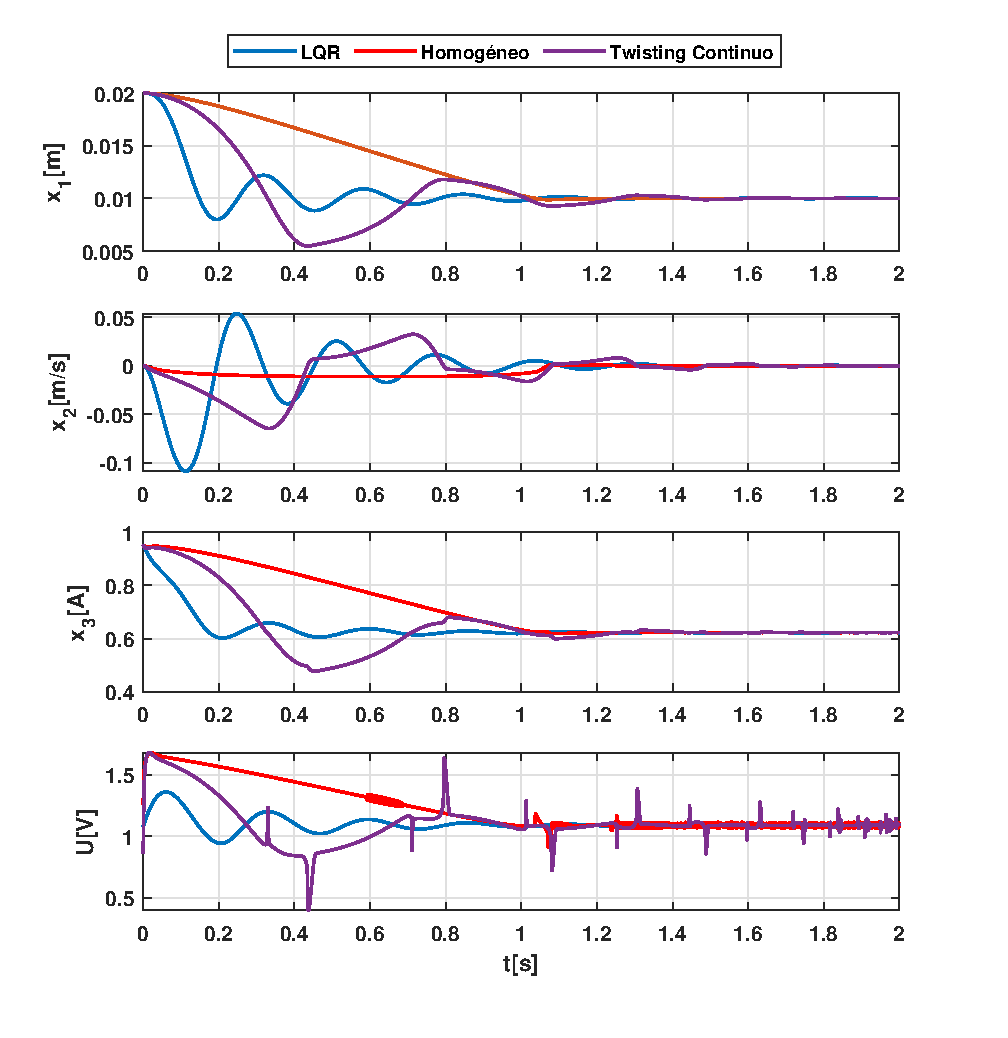
\includegraphics[scale=0.55]{xu_3o_c3o.eps}
\caption{Comportamiento del sistema debido a controladores de 3er orden con $f(t)=0$}
\end{figure}
\\
Se puede ver que con los 3 controladores se alcanz\'o el punto de operaci\'on pero con ciertas diferencias en las trayectorias que siguen los estados, el comportamiento debido a los controladores lineales es m\'as r\'apido y hay convergencia en tiempo finito.


\subsubsection*{Con Perturbaciones}
Para este caso se incluyeron perturbaciones (variables en el tiempo), en concreto fue una suma de senos y cosenos $f(t)=0.5(sen(t)+cos(2t)+1)$ cuya gr\'afica se muestra en la Figura 3. 
\begin{figure}[!h]
\centering
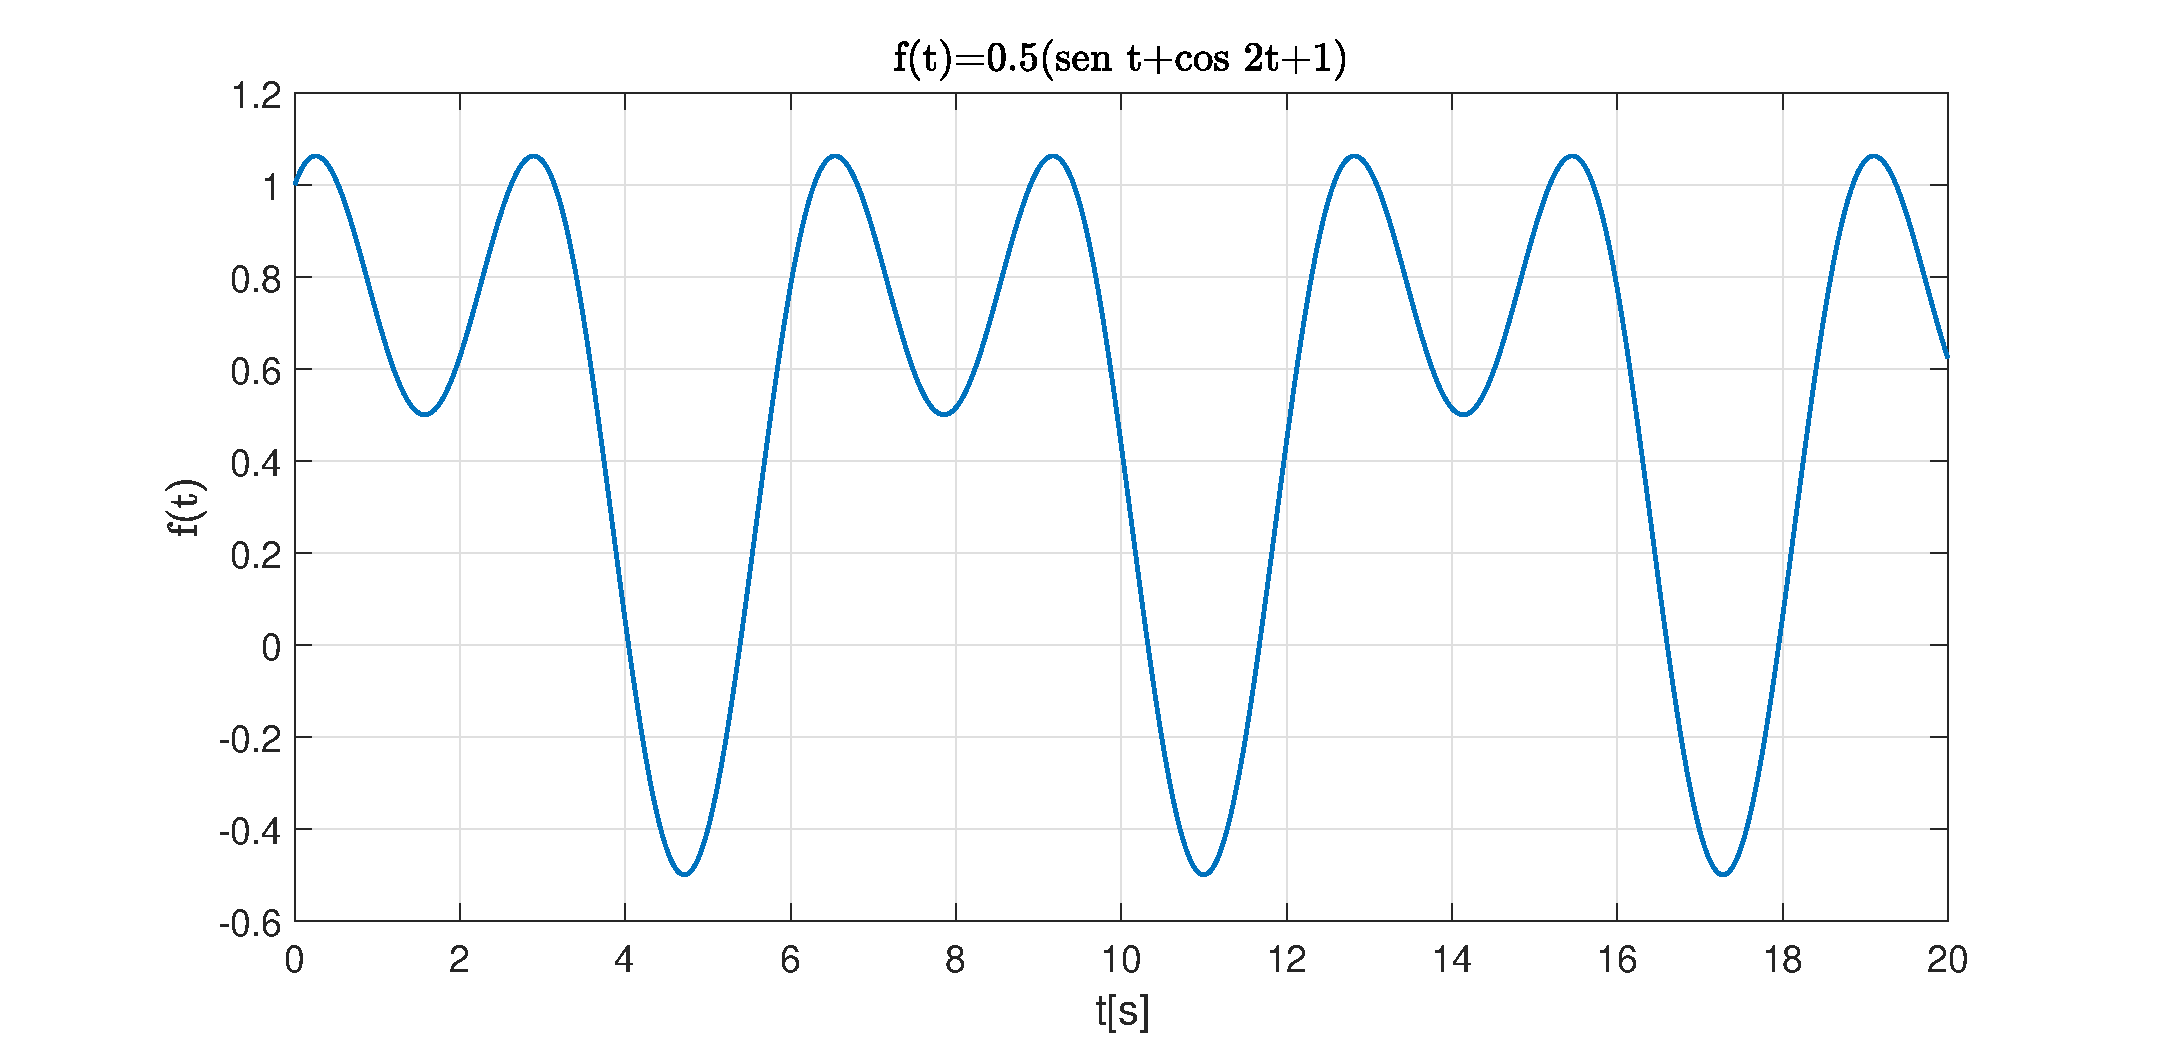
\includegraphics[scale=0.26]{pv.eps}
\caption{Perturbaci\'on variable $f(t)=0.5(sen(t)+cos(2t)+1)$}
\end{figure}
\\
\\
\\
\\
\\
\\
\\
Las trayectorias que siguieron los estados y la entrada con este cambio se muestran en la Figura 4.
\begin{figure}[!h]
\centering
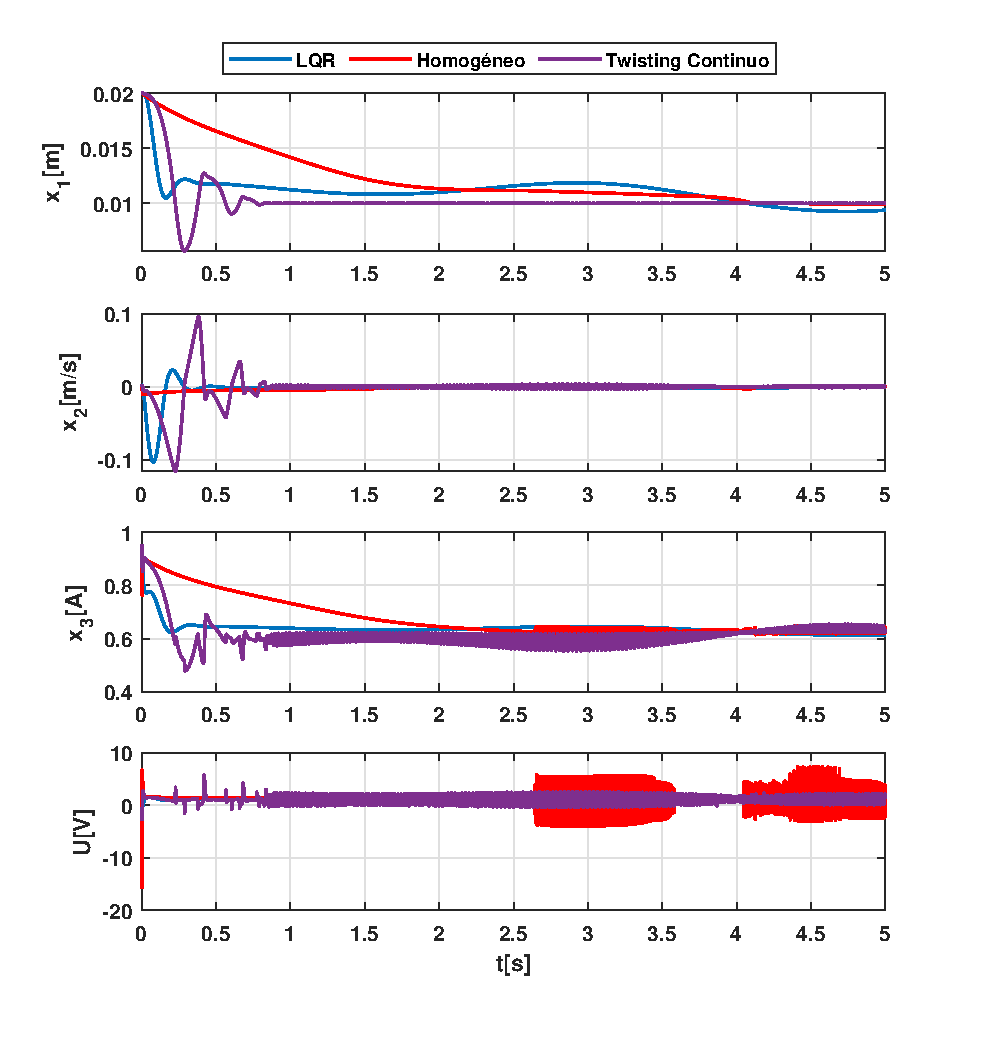
\includegraphics[scale=0.55]{xu_3o_c3o_pv.eps}
\caption{Comportamiento del sistema debido a controladores de 3er orden con $f(t)=0.5(sen(t)+cos(2t)+1)$}
\end{figure}
\\
Aqu\'i se pudo ver que el controlador PID no es capaz de rechazar esas perturbaciones pero tampoco el controlador Homog\'eneo (aunque lo hace mejor), el \'unico que si pudo manejar las perturbaciones es el controlador Twisting Continuo.

\section{Sistema de 2do Orden}
Aprovechando que el transitorio de la din\'amica el\'ectrica del sistema es estable y m\'as r\'apida que la mec\'anica lo siguiente fue hacer una reducci\'on del sistema tomando solo dicha parte mec\'anica del sistema original o de 3er orden, obteniendo un sistema de 2do orden formado por los estados $x_1$  y $x_2$ por lo que $x_3$ no se consider\'o para los c\'alculos, esto fue con el objetivo de analizar su comportamiento y dise\~narle controladores.
\subsection*{Representaci\'on del Sistema}
Con base en la ecuaciones de estado del sistema de 3er orden para $x_2$:
$$\dot{x_2}=-\dfrac{k}{m}x_2 -g  +\dfrac{aL_0x_3^{2}}{2m(a+x_1)^{2}}$$

se tom\'o al termino $L_0x_3^{2}$ como la nueva entrada de control $u$ y solo se consideraron las ecuaciones para $\dot{x_1}$ y $\dot{x_2}$ obteniendo la siguiente representaci\'on:
$$
\dot{x_1}=x_2 
$$
$$
\dot{x_2}=-\dfrac{k}{m}x_2  -g  +\dfrac{a}{2m(a+x_1)^{2}}\cdot u
$$
Con un punto de operaci\'on $X_d$ debido a una $U_d$ al cual llevar al sistema, tal que $\dot{x}=0$:
$$
X_{d}=\begin{bmatrix}
X_{1_{D}} \\ 0  
\end{bmatrix}
$$
$$
U_{d}=\begin{matrix}
\dfrac{2mg}{a}(a+X_{1_{D}})^{2}
\end{matrix}
$$
Donde $X_{1_{D}}$ es la distancia a la cual queremos situar el objeto, manteniendo $0.01[m]$ se obtuvo:
$$
X_{d}=\begin{bmatrix}
0.01 \\ 0  
\end{bmatrix}
$$
$$
U_{d}=\begin{matrix}
0.0948
\end{matrix}
$$

\subsection*{Control del Sistema}
Al igual que en el sistema de 3er orden, para el de 2do orden se dise\~n\'o un controlador LQR de la forma $u=-K(x-X_{d})+U_{d}$.

Por lo que con ayuda de MATLAB se tuvo que realizar una linealizaci\'on del sistema para obtener una representaci\'on $\dot{x}=Ax+Bu$, $y=Cx+Du$, los valores num\'ericos de las matrices $A$, $B$, $C$ y $D$ que se obtuvieron son los siguientes:
$$A=\begin{bmatrix}
0 & 1 \\
-1044.1495 & -0.0831\\
\end{bmatrix}$$

$$
B= \begin{bmatrix}
0  \\ 103.4836
\end{bmatrix}
$$
$$
C= \begin{bmatrix}
1 & 0 \\ 
0 & 1 \\ 
\end{bmatrix}
$$
$$
D=\begin{bmatrix}
0 \\ 0
\end{bmatrix}
$$
Lo siguiente fue comprobar la controlabilidad del sistema, igualmente con la ayuda de MATLAB, una vez que se supo que el sistema es completamente controlable, se calcularon las ganancias para el controlador.

Los siguientes controladores fueron un PD de la forma:
\begin{equation*}
\begin{split}
 u&=-k_1e-k_2x_2\\
 e&=x_1-X_{1_{D}}
\end{split}
\end{equation*}

Y un PID de la forma:
\begin{equation*}
\begin{split}
 u&=-k_1e-k_2\int_{0}^{t}edt-k_3x_2\\
 e&=x_1-X_{1_{D}}
\end{split}
\end{equation*}

Con los siguientes controladores primero se llev\'o al sistema a una forma de cadena de integradores por lo que se sigui\'o un procedimiento parecido al que se hab\'ia utilizado en el sistema de 3er orden pero con la ventaja que el sistema de 2do orden ya se encontraba en una forma af\'in al control, debido a ello se implement\'o un control por linealizaci\'on exacta $u=g(x)^{-1}(\nu-f(x))$ sin necesidad de hacer una transformaci\'on previa, $\nu$ puede ser un control lineal o no lineal.

Donde:
$$
f(x)= - \dfrac{k}{m} x_2 - g
$$
$$
g(x)=\dfrac{a}{2m(a+x_1)^{2}}
$$
El primer controlador que se dise\~n\'o fue:
\begin{equation*}
\begin{split}
 u&=g^{-1}(x)(\nu-f(x))\\
 \nu&=-k_1\lceil x_1-X_{1_{D}} \rfloor ^{\frac{1}{3}}-k_2\lceil x_2 \rfloor ^{\frac{1}{3}}
\end{split}
\end{equation*}
Donde $\nu$ es un controlador homog\'eneo.

Y el segundo controlador que se dise\~n\'o fue:
\begin{equation*}
\begin{split}
 u&=g^{-1}(x)(\nu-f(x))\\
 \nu&=-k_1\lceil x_1-X_{1_{D}} \rfloor ^{\frac{1}{3}}-k_2\lceil x_2 \rfloor ^{\frac{1}{2}}+\eta \\
\dot{\eta}&=-k_3\lceil x_1-X_{1_{D}} \rfloor ^{0}-k_4\lceil x_2 \rfloor ^{0} 
\end{split}
\end{equation*}
Donde $\nu$ es un controlador Twisting continuo.

\section{Control del sistema de 3er Orden mediante controladores de 2do Orden}
\subsection*{Sin Perturbaciones}
Todo lo realizado en la secci\'on anterior se hizo con el objetivo de familiarizarse con las caracter\'isticas y el comportamiento del sistema para poder aprovecharlas y facilitar la tarea del control, esto quiere decir usar los controladores de segundo orden (los dise\~nados para el sistema de 2do orden) y con ellos controlar al sistema de 3er orden u original, por lo que se le estar\'ia llevando al punto de operaci\'on deseado con la informaci\'on de solo el estado $x_1$ y $x_2$.

Para lograr ese objetivo lo primero que se hizo fue implementar directamente un control por linealizaci\'on exacta $u=g(x)^{-1}(\nu-f(x))$ con:
$$
f(x)= - \dfrac{k}{m} x_2 - g
$$
$$
g(x)=\dfrac{a}{2m(a+x_1)^{2}}\cdot
$$
Esto se pudo hacer, como se hab\'ia mencionado antes, debido a que el transitorio de la din\'amica de la parte el\'ectrica del sistema es estable y se desvanece muy r\'apido dejandonos pr\'acticamente con un sistema de 2do orden en el que se encuentra la informaci\'on de la parte mec\'anica m\'as lenta que domina el comportamiento transitorio del sistema de 3er orden.

Como solo se controlaron los estados $x_1$ y $x_2$ se hicieron ajustes en las ganancias de los controladores de 2do orden empleados para compensar que no se tom\'o en cuenta la parte el\'ectrica.

El primer controlador que se utiliz\'o fue:
\begin{equation*}
\begin{split}
 u&=g^{-1}(x)(\nu-f(x))\\
 \nu&=-k_1e-k_2x_2 \\
e&=x_1-X_{1_{D}} 
\end{split}
\end{equation*}
Donde $\nu$ es un control PD.

El segundo controlador que se utiliz\'o fue:
\begin{equation*}
\begin{split}
 u&=g^{-1}(x)(\nu-f(x))\\
 \nu&=-k_1e-k_2\int_{0}^{t}edt-k_3x_2 \\
e&=x_1-X_{1_{D}} 
\end{split}
\end{equation*}
Donde $\nu$ es un control PID.

El tercer controlador que se utiliz\'o fue:
\begin{equation*}
\begin{split}
 u&=g^{-1}(x)(\nu-f(x))\\
 \nu&=-k_1\lceil x_1-X_{1_{D}} \rfloor ^{\frac{1}{3}}-k_2\lceil x_2 \rfloor ^{\frac{1}{3}}
\end{split}
\end{equation*}
Donde $\nu$ es un control homog\'eneo.


El \'ultimo controlador que se utiliz\'o fue:
\begin{equation*}
\begin{split}
 u&=g^{-1}(x)(\nu-f(x))\\
 \nu&=-k_1\lceil x_1-X_{1_{D}} \rfloor ^{\frac{1}{3}}-k_2\lceil x_2 \rfloor ^{\frac{1}{2}}+\eta \\
\dot{\eta}&=-k_3\lceil x_1-X_{1_{D}} \rfloor ^{0}-k_4\lceil x_2 \rfloor ^{0} 
\end{split}
\end{equation*}
Donde $\nu$ es un control Twisting continuo.

Sin considerar perturbaciones los resultados que se obtuvieron se muestran en la Figura 5.
\begin{figure}[!h]
\centering
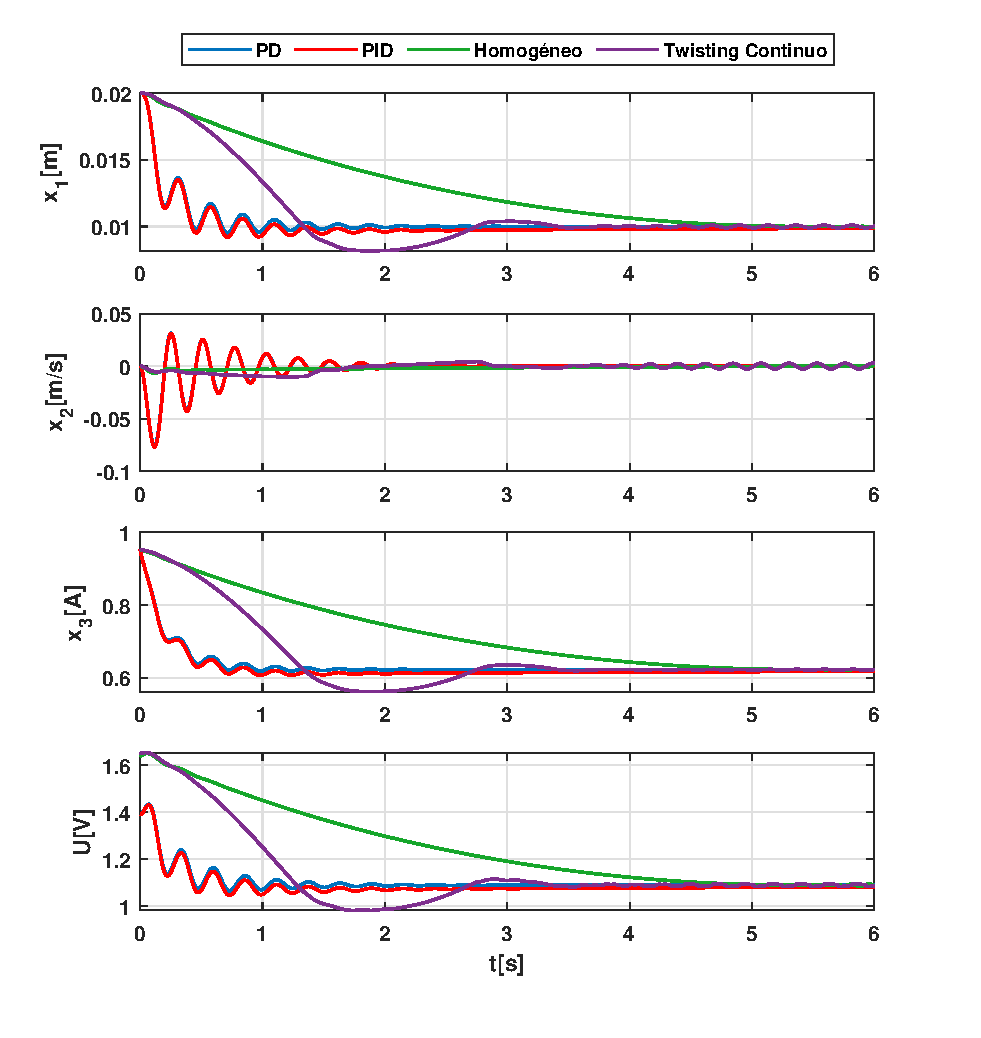
\includegraphics[scale=0.55]{xu_3o_c2o.eps}
\caption{Comportamiento del sistema debido a controladores de 2do Orden con $f(t)=0$}
\end{figure}
\\
Se observ\'o que estos controladores tambien son capaces de llevar al sistema al punto de operaci\'on o cuando menos a una regi\'on cercana a \'el, pero tomandonse m\'as tiempo para ello.
\subsection*{Con Perturbaciones}
Lo siguiente que se hizo fue cambiar a perturbaciones constantes y variables eligiendo $f(t)=0.5$ y $f(t)=0.5(sen(t)+cos(2t)+1)$, el como respondieron los estados del sistema y su entrada se muestran en las Figuras 6 y 7 respectivamente.
\begin{figure}[!h]
\centering
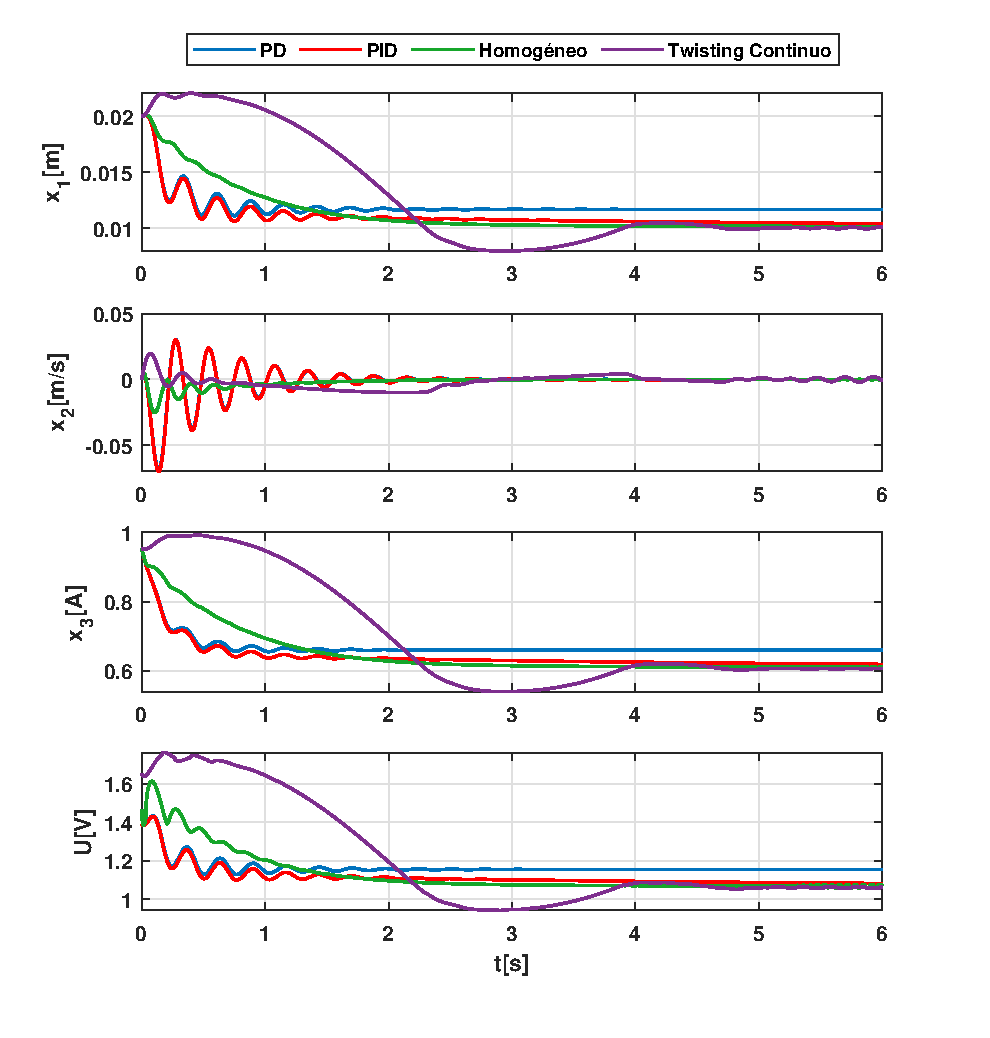
\includegraphics[scale=0.55]{xu_3o_c2o_pc.eps}
\caption{Comportamiento del sistema debido a controladores de 2do Orden con  $f(t)=0.5$}
\end{figure}
\\
\\
\\
\\
\\
\\
\\
\\
\\
\\
\\
\\
\\
\\
\\
\\
\\
En este caso el controlador PD fue el \'unico incapaz de llevar al sistema al punto de operaci\'on, siempre hubo un error en estado estacionario, pudo estabilizar al sistema pero los estados quedaban muy lejos de los valores deseados.
\begin{figure}[!h]
\centering
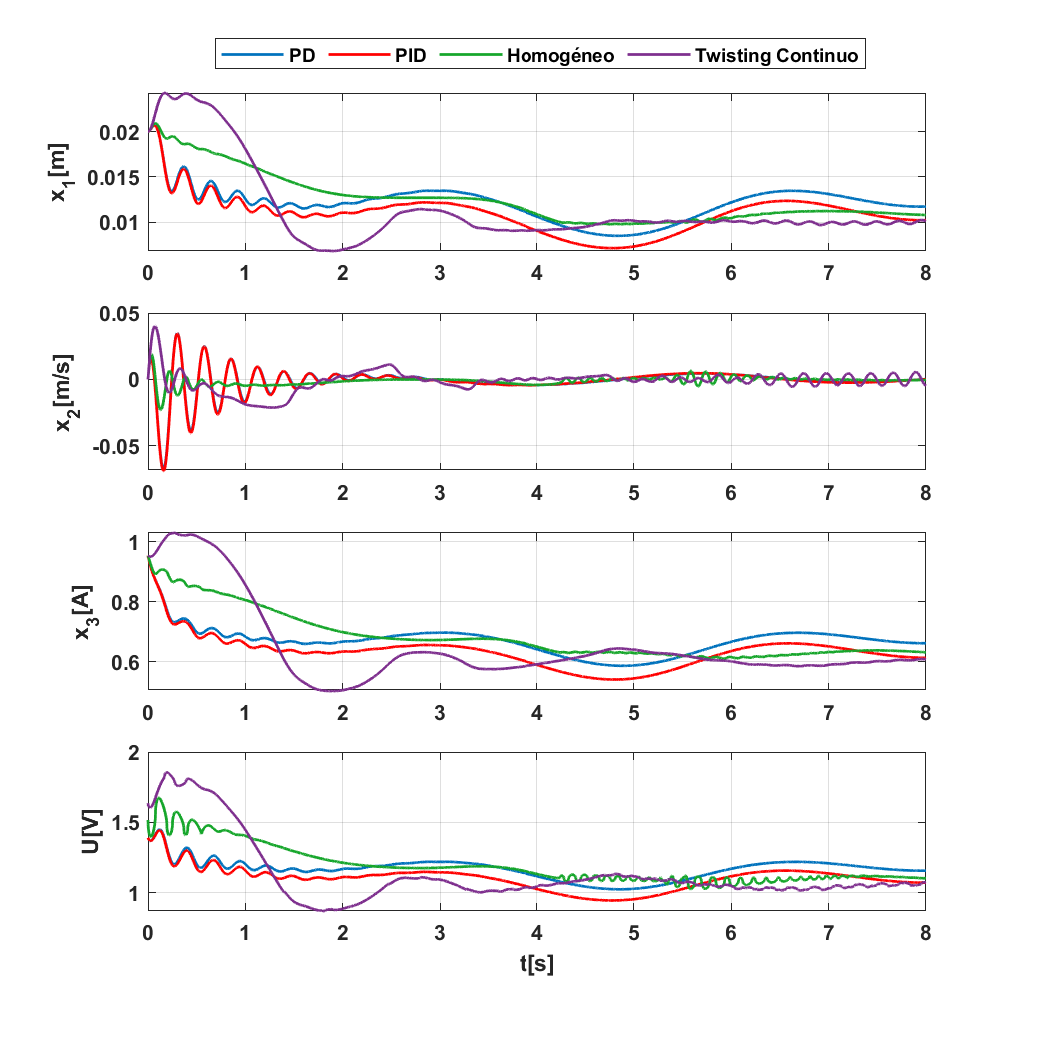
\includegraphics[scale=0.55]{xu_3o_c2o_pv.eps}
\caption{Comportamiento del Sistema debido a controladores 2do Orden con $f(t)=0.5(sen(t)+cos(2t)+1)$}
\end{figure}
\\
\\
\\
\\
\\
\\
\\
\\
\\
\\
\\
\\
\\
\\
\\
\\
\\
\\
\\
\\
\\
\\
\\
\\
Aqu\'i solo el Controlador Twisting Continuo pudo llevar al sistema a una regi\'on cercana del punto de operaci\'on, fue quien mejor manejo la perturbaci\'on variable, el PID ya no pudo rechazarla, tampoco el controlador Homog\'eneo pero tuvo un desempe\~no no tan malo.
\section*{Comparaci\'on entre controladores}
Como se pud\'o observar en las gr\'aficas mostradas antes, al aplicar controladores lineal y no lineales de 2do y 3er orden al sistema original sin perturbaciones se logr\'o alcanzar y permanecer en el punto de operaci\'on establecido pero con diferencias en el desempe\~no entre las diferentes t\'ecnicas empleadas por lo que con base en ciertos criterios y dependiendo de la aplicaci\'on asi como de los recursos disponibles surgir\'an tanto ventajas como desventajas.

Una forma de hacer m\'as notorias estas diferencias de desempe\~no fue aplicar perturbaciones constantes y variables para ver la robustez de los controladores empleados pero siempre con controladores del mismo orden, por lo que lo siguiente fue contrastar en una misma gr\'afica el comportamiento de los estados y la entrada del sistema debido a controladores de 2do Orden y su "contraparte" de 3er Orden, recordando que se quiere llegar a:
\\
\\
\\
\\
$$
X_{D}=\begin{bmatrix}
0.01 \\ 0 \\ 0.6222 
\end{bmatrix}
$$
$$
U_{d}=\begin{matrix}
1.0888
\end{matrix}
$$

\subsection*{Controladores Lineales}
Se compararon los estados y entrada del sistema debido a controladores lineales de 2do Orden como el PD y el PID adem\'as del LQR de 3er Orden con perturbaciones constantes y variables, los resultados obtenidos se muestran en las Figuras 8 y 9 respectivamente.
\begin{figure}[!h]
\centering
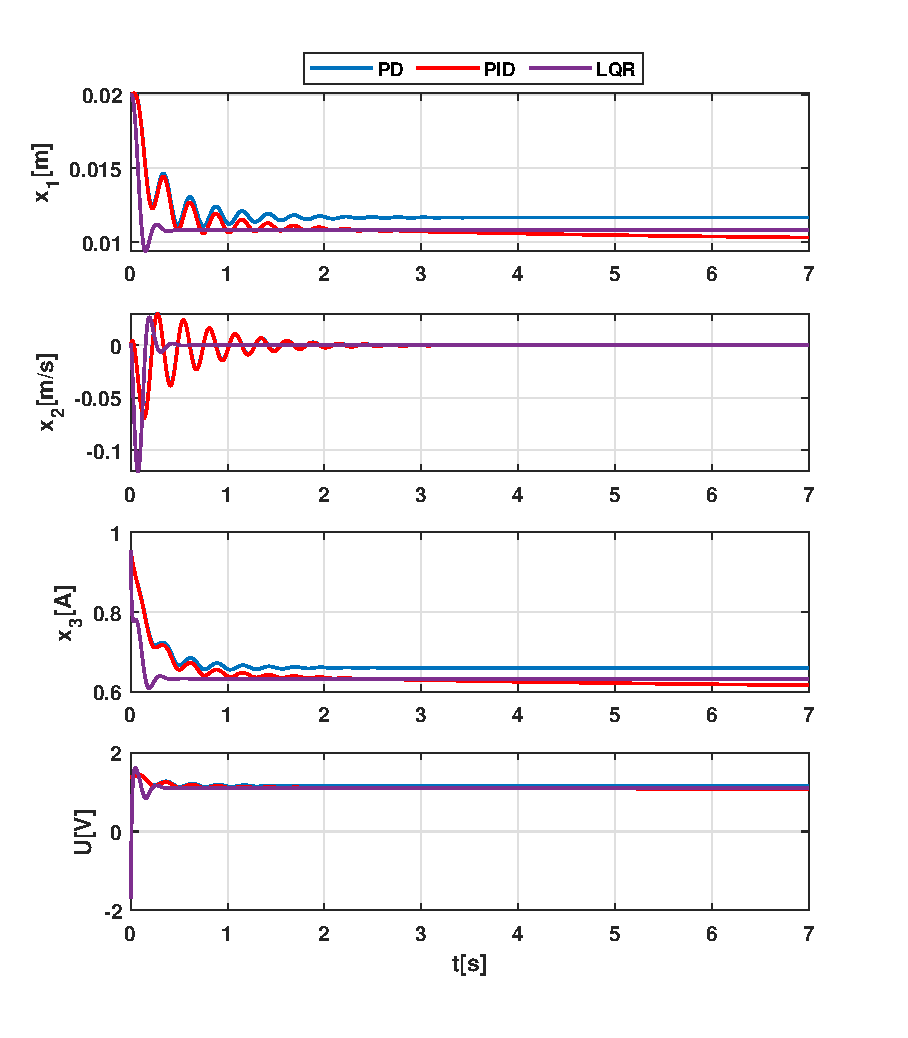
\includegraphics[scale=0.55]{xu_3o_pdpidlqr_pc.eps}
\caption{Comportamiento del sistema debido a controladores lineales de 2do y 3er orden con $f(t)=0.5$}
\end{figure}
\\
Como se hab\'ia observado antes, el controlador PID fue el \'unico capaz de lidiar con la perturbaci\'on constante, ni siquiera el LQR (aunque fue el m\'as r\'apido en estabilizar al sistema). 
\begin{figure}[!h]
\centering
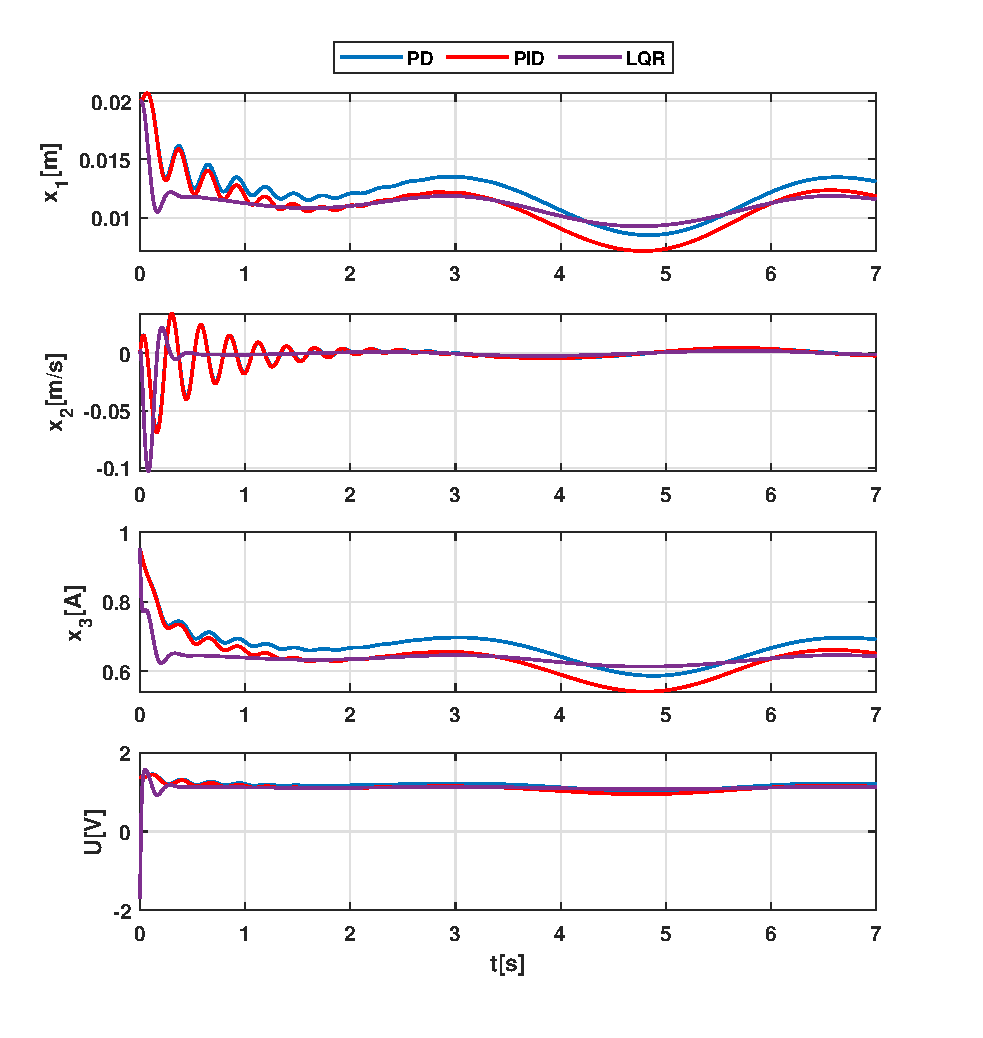
\includegraphics[scale=0.55]{xu_3o_pdpidlqr_pv.eps}
\caption{Comportamiento del sistema debido a controladores lineales de 2do y 3er orden con $f(t)=0.5(sen(t)+cos(2t)+1)$}
\end{figure}
\\
\\
\\
\\
\\
\\
\\
\\
\\
\\

En esta situaci\'on ya ninguno de los 3 controladores fue capaz de lidiar de buena manera con la perturbaci\'on variable.
\subsection*{Controladores no Lineales}
Por \'ultimo se compararon los estados y entrada del sistema debido a controladores no lineales de 2do y 3er Orden como el Homog\'eneo y Twisting Continuo con perturbaciones constantes y variables, los resultados obtenidos se muestran en las figuras 10 a 13.
\begin{figure}[!h]
\centering
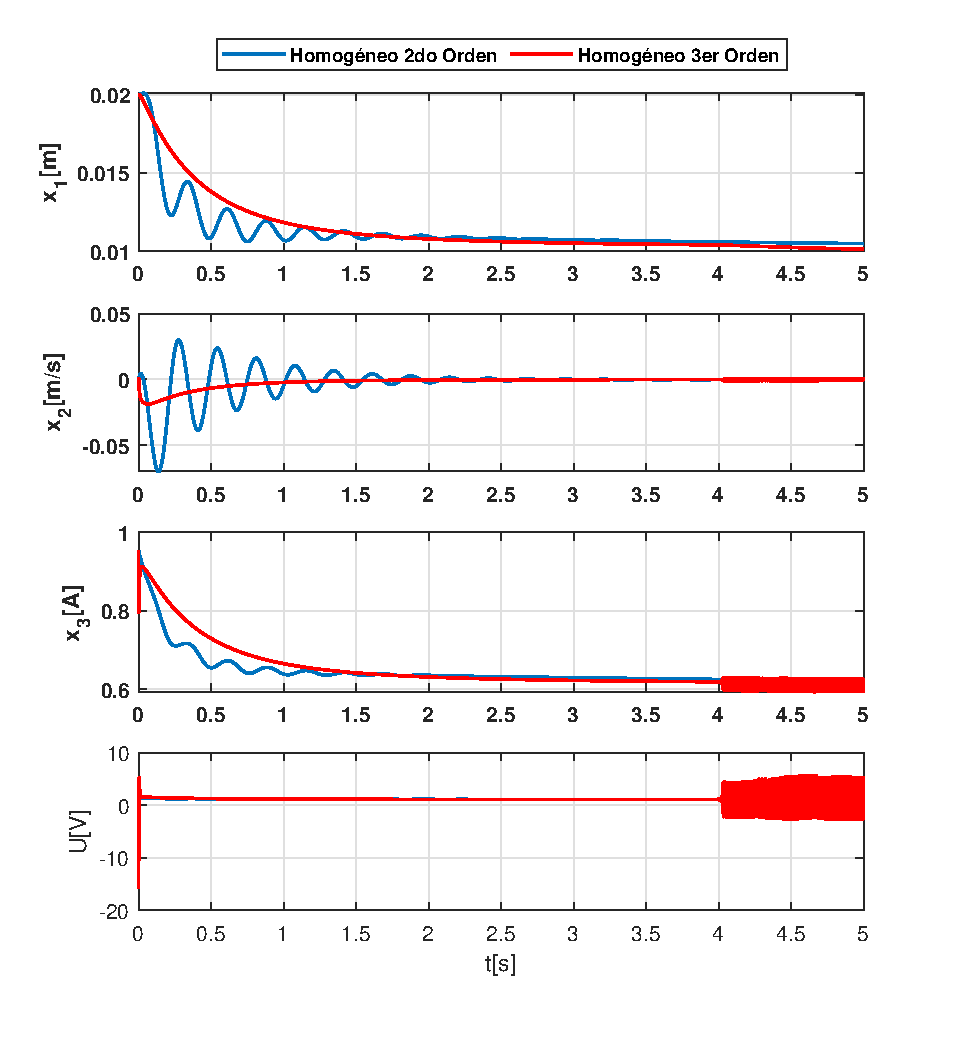
\includegraphics[scale=0.55]{xu_3o_h23o_pc.eps}
\caption{Comportamiento del sistema debido a controladores Homog\'eneos de 2do y 3er Orden con $f(t)=0.5$}
\end{figure}
\\
\\
\\
\\
\\
\\
\\
\\
\\
\\
\\
\\
\\
\\
\\
\\
\\
Como se puede ver en las gr\'aficas el controlador Homog\'eneo de 3er Orden tuvo un mejor desempe\~no al manejar la perturbaci\'on constante, pero eso no quiere decir que no sea aceptable el controlador de 2do Orden, una ventaja que tiene es que la se\~nal de control que produce no es tan abrupta como la del controlador de 3er Orden.
\begin{figure}[!h]
\centering
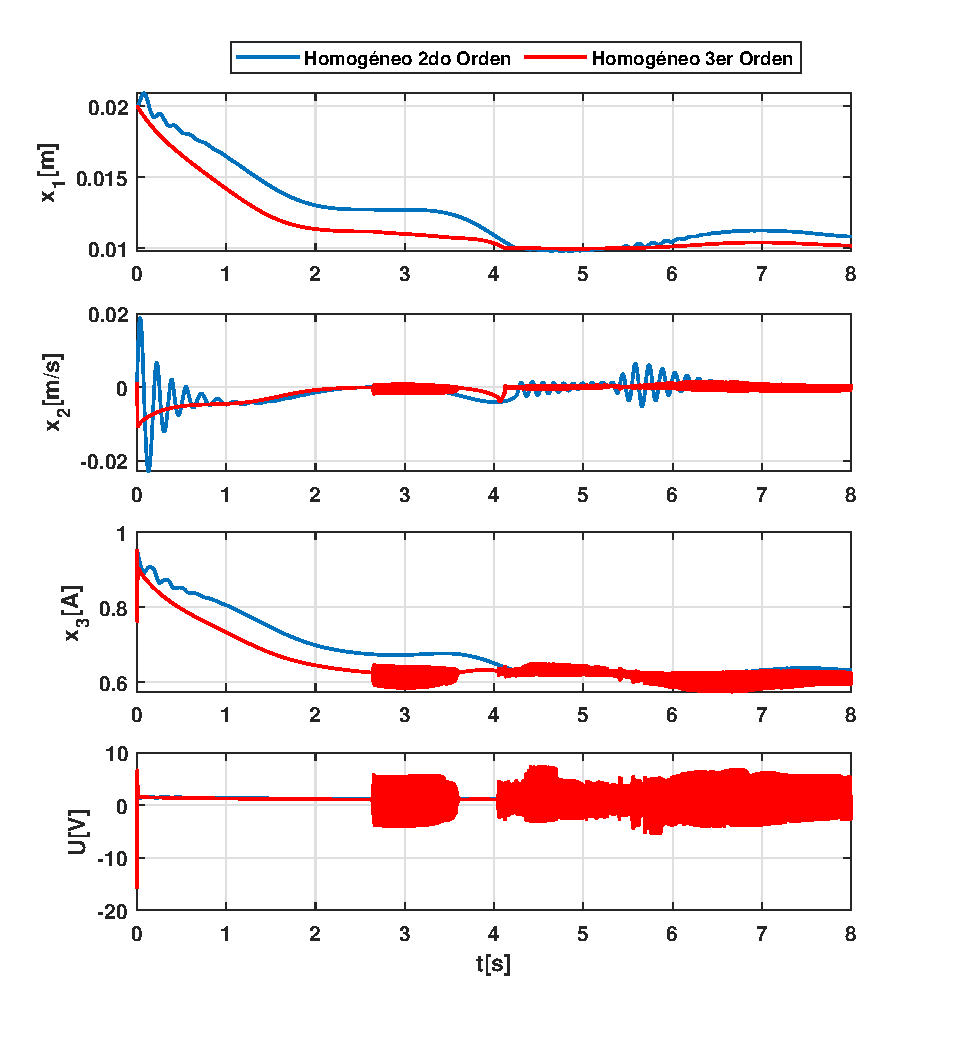
\includegraphics[scale=0.55]{xu_3o_h23o_pv.eps}
\caption{Comportamiento del sistema debido a controladores Homog\'eneos de 2do y 3er Orden con $f(t)=0.5(sen(t)+cos(2t)+1$}
\end{figure}
\\
\\
\\
\\
\\
\\
\\
\\
\\
\\
\\
\\
\\
\\
\\
\\
\\
\\
\\
\\
\\
\\
\\
Ninguno de los 2 controladores pudo rechazar de buena manera la perturbaci\'on variable, sin embargo el controlador de 3er Orden tuvo un mejor desempe\~no.
\begin{figure}[!h]
\centering
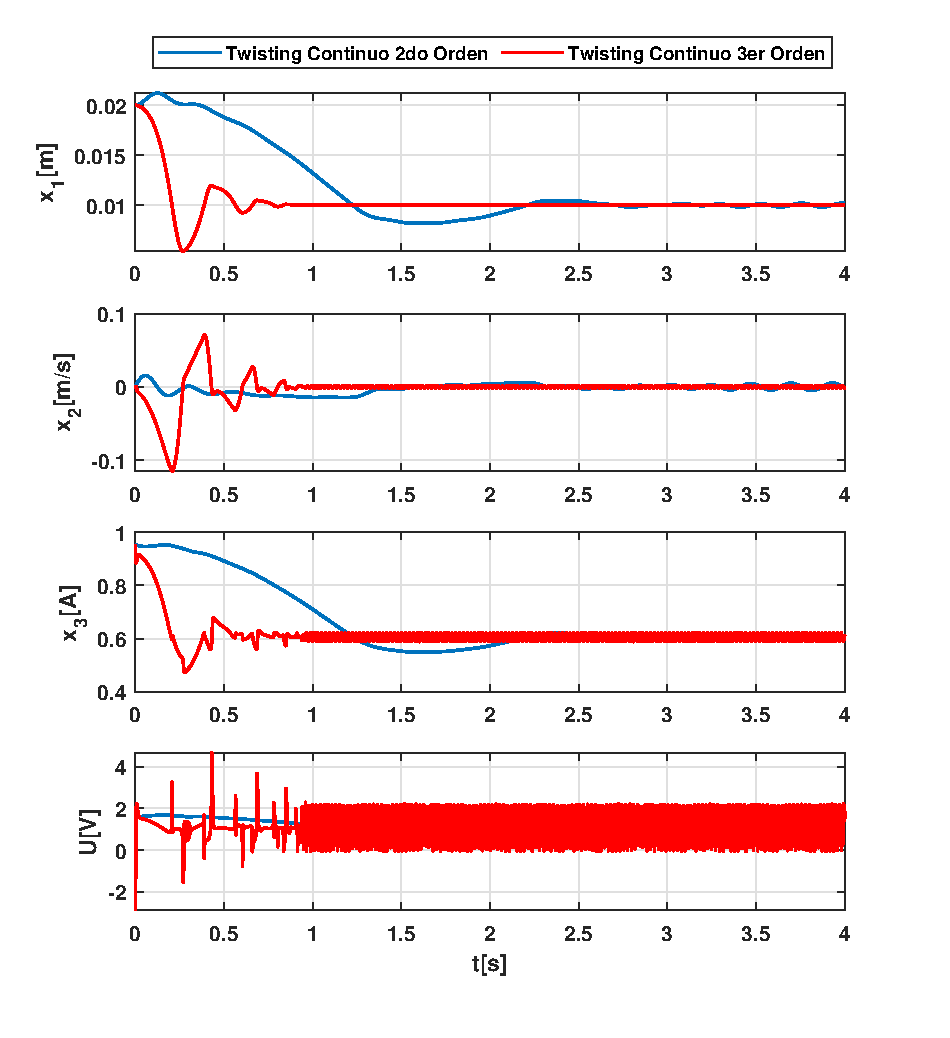
\includegraphics[scale=0.55]{xu_3o_tc23o_pc.eps}
\caption{Comportamiento del sistema debido a controladores Twisting Continuos de 2do y 3er Orden con $f(t)=0.5$}
\end{figure}
\begin{figure}[!h]
\centering
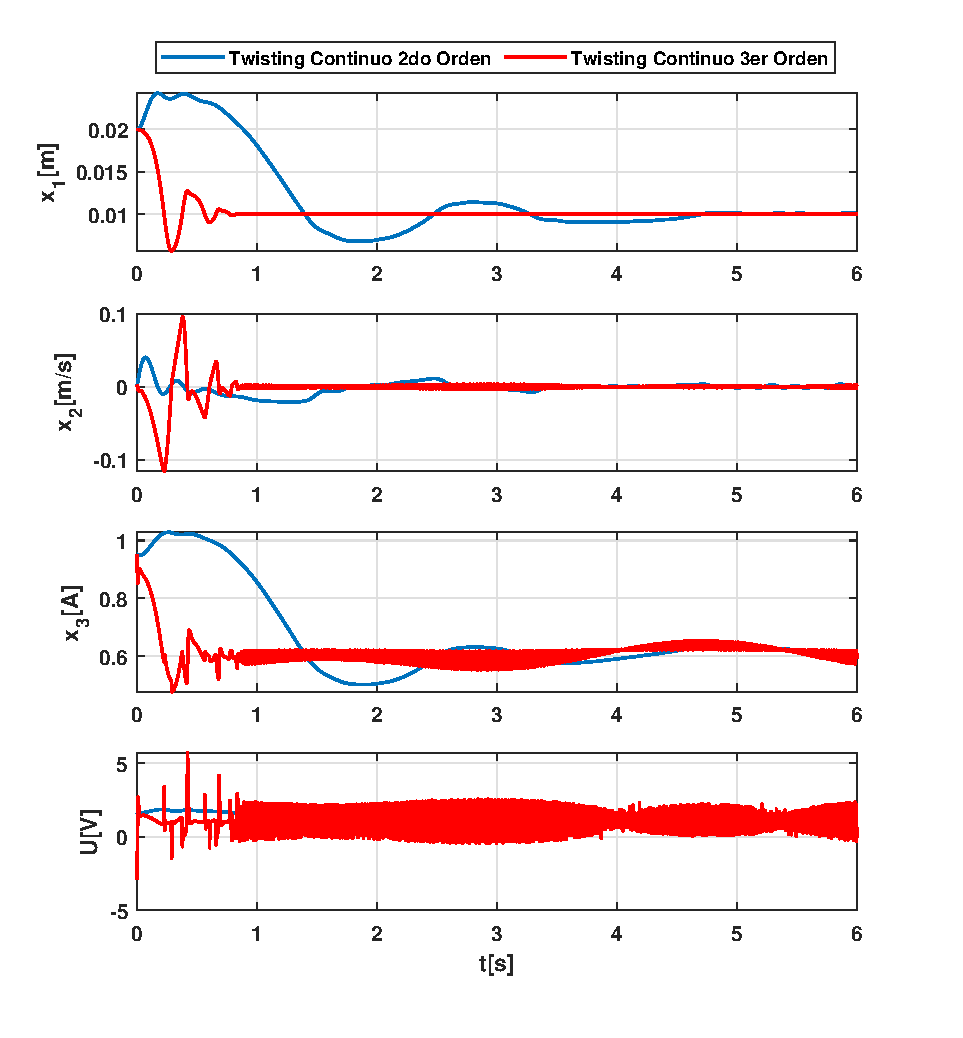
\includegraphics[scale=0.55]{xu_3o_tc23o_pv.eps}
\caption{Comportamiento del sistema debido a controladores Twisting Continuos de 2do y 3er Orden con $f(t)=0.5(sen(t)+cos(2t)+1$}
\end{figure}
\\
\\
\\
\\
\\
\\
\\
\\
\\
\\
\\
\\
\\
\\
\\
\\
\\
\\
\\
\\
\\
\\
\\
\\
\\
Tanto con perturbaciones variables como constantes se tuvo un comportamiento aceptable, los controladores son capaces de rechazarlas pero el controlador de 3er Orden hace que el sistema converga al punto de operaci\'on m\'as r\'apido pero produciendo se\~nales de control muy abruptas.

\section{Conclusiones}
Se pudieron observar diferencias como un mayor tiempo de convergencia de los estados y mayor comportamiento oscilatorio en las trayectorias del sistema debido al controlador de 2do Orden respecto del 3er Orden ya que al estado $x_3$ se le deja libre, no se le controla, se tiene que esperar a que converga a su estado estacionario para que $x_1$ y $x_2$ puedan converger tambien, antes de ello solo se les mantiene acotados.

Otra forma de interpretar estas diferencias es haciendo distinci\'on entre controladores lineales y no lineales, en las que una de las m\'as importantes fue la capacidad de rechazar perturbaciones tanto constantes como variables, dicha capacidad fue mejor entre los controladores no lineales  adem\'as de hicieron que los estados del sistema tengan una mayor rapidez de convergencia al punto de operaci\'on, pero con la desventaja que por ejemplo comparandolo con el PID produc\'ian se\~nales de control m\'as accidentes y en el caso del controlador Homog\'eneo con saltos muy pronunciados(tambien en el LQR pero eso fue debido a las altas ganancias que se eligieron).




\section{Referencias}
\begin{itemize}
\item Khalil, H.. (2002). Nonlinear Systems. USA: Prentice Hall.
\item Moore, J.. (1989). Optimal Control Linear Quadratic Method. USA: Prentice Hall. 
\item Slotine, J. J. E., \& Li, W. (1991). Applied nonlinear control (Vol. 199, No. 1). Englewood Cliffs, NJ: Prentice hall.
\item Williams, R. L., \& Lawrence, D. A. (2007). Linear state-space control systems. John Wiley \& Sons.
\end{itemize}

\bibliographystyle{apalike} 
\bibliography{biblio} 
\end{document}
